\section{Methodology}
    % Über Bau des Spektrometers erzählen
    % Formeln erklären
    % Argumentieren warum wir grating constant vom internet nehmen

    To build the spectrometer, cardboard, tape, two razor blades, a CD and a camera (ideally wide angle) is needed.
    The less reflective the cardboard is, the better the results are going to be.
    Build a tube with the cardboard and attach the two razor blades to one end, leaving just a small slit of about 0.2 mm for light to enter.
    Remove the reflective foil off the CD using a cutter and tape and cut out a piece of the transparent part of the size of the cardboard tube.
    tape it to the open end of the tube.
    Now attach the camera to the same side.
    make sure no light enters the apparatus except through the slit.

    If held in the direction of a light source, a diffraction pattern, showing the spectrum of the different wavelengths, is visible on the camera.
    The formula relating the distance of the maxima of different orders to the wavelength of the light entering the spectrometer is given in equation~\eqref{eq_interference}.

    \begin{align}
        p \lambda = g \sin(\phi) \label{eq_interference}
    \end{align}

    $p$ is an integer called the order number. For the first visible maximum, $p$ is equal to $1$, for the second maximum $p = 2$ and so on.
    $\lambda$ is the wavelength of the light.
    The grating constant $g$ is dependent on the distance between the slits in the grating.
    Hence this constant is not the same for different kinds of CDs or DVDs.
    the last variable is the angle $\phi$ in the triangle of the maximum of zero and $p^{th}$ order and the spot where the light passes through the grating, measured at the grating.
    Trigonometry gives the relation in equation~\eqref{eq_phi}, which is visible in the figure~\ref{fig_phi}.
    
    \begin{align}
        \tan(\phi) = \frac{x_p}{d} \label{eq_phi}
    \end{align}

    \begin{figure}[H]
        \centering
        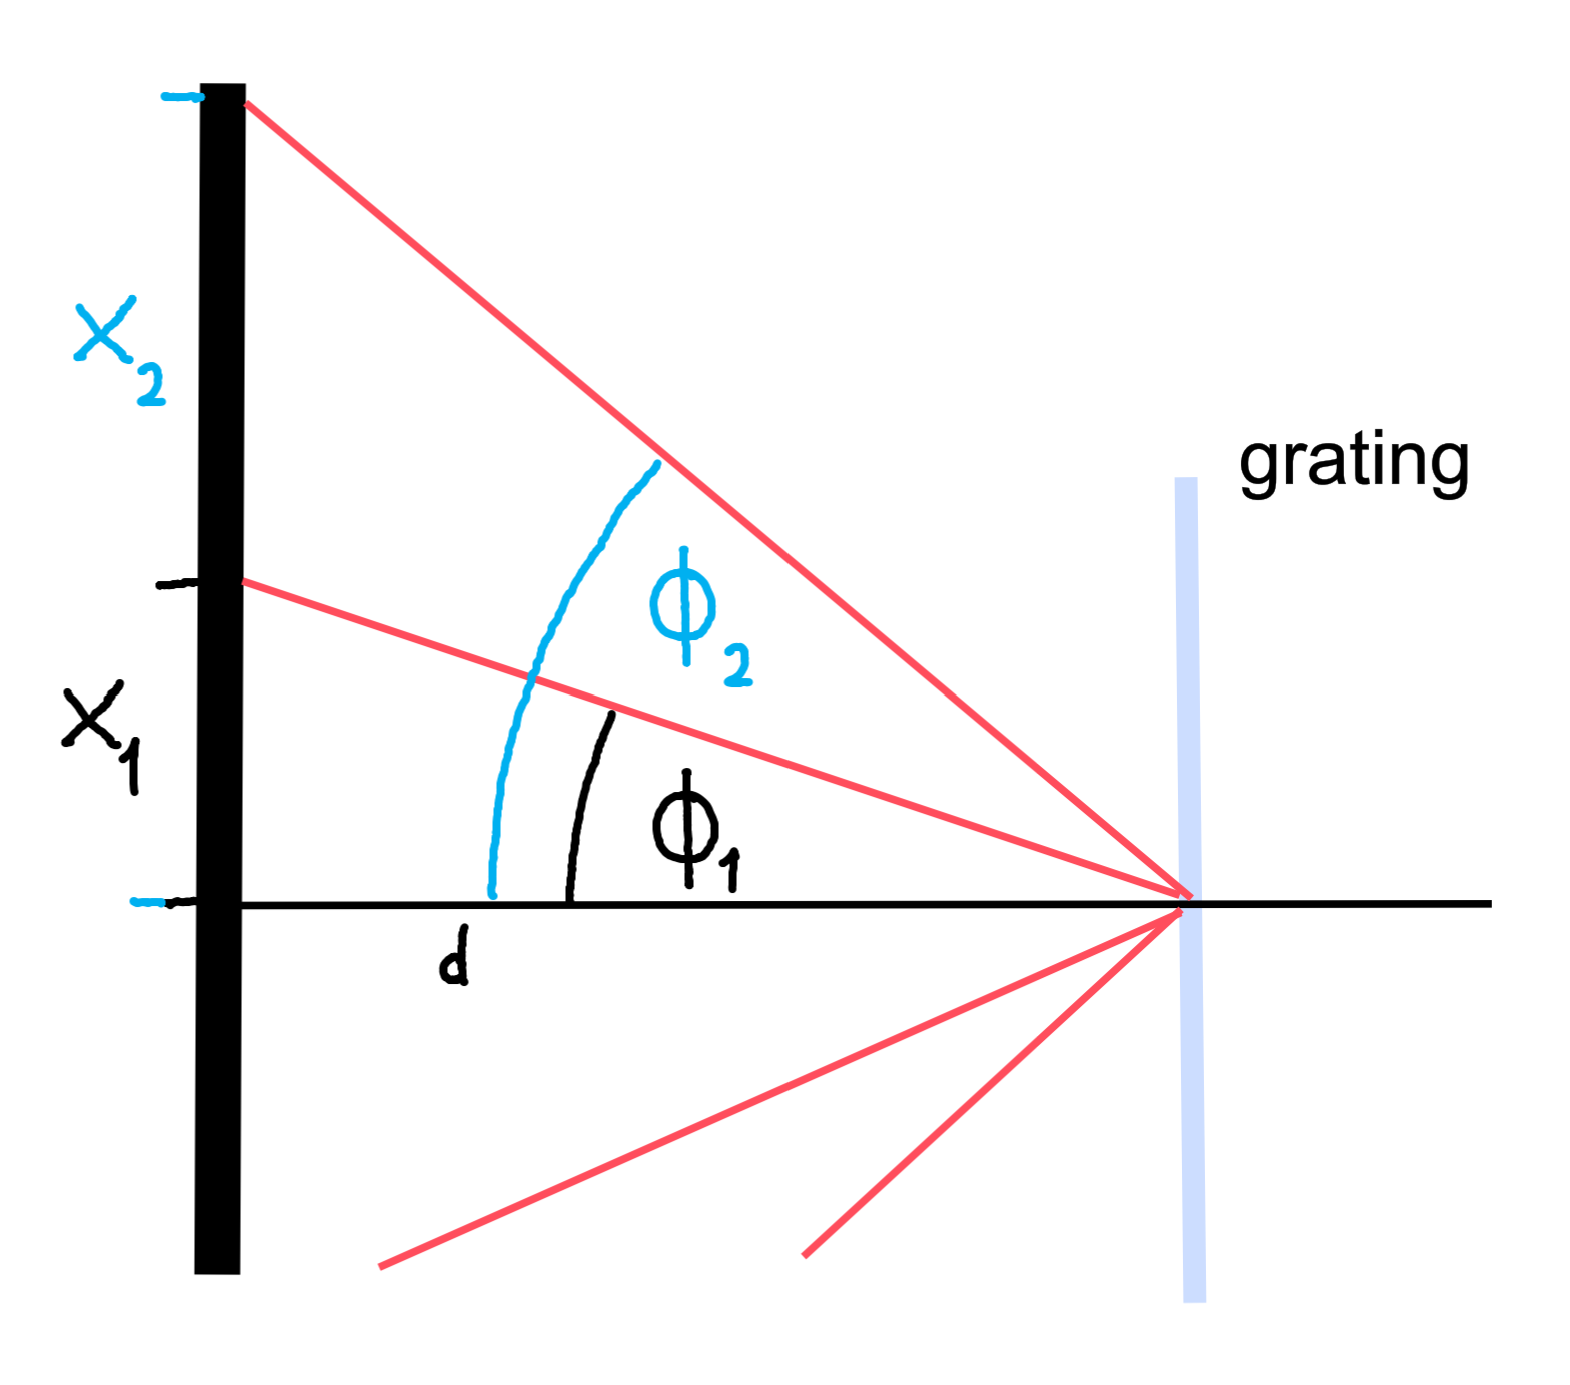
\includegraphics[scale = 0.7]{src/images/angle_phi.png}
        \caption{Visualization of the location of the angle $\phi$ referred to in equation~\eqref{eq_interference}.
        The first and second maximum of one certain wavelength is shown, so monochromatic light would be needed to reproduce this hypothetical situation.}
        \label{fig_phi}
    \end{figure}

    In our test case, we assumed a grating constant $g = 1.514 \mu m$ \cite{src_grating_constant} as we did not have a monochromatic light source at hand to determine the grating constant of our CD.
    Next, we calculated the distance between the CD and the camera to calibrate our spectrometer using a first measurement and by choosing a certain colour and its corresponding wavelength by eye.

    Now, having a calibrated and working spectrometer, we did multiple measurements of different light sources.

    \subsection{Different types of light sources}

    Artificial light sources can be roughly categorized in the following groups:

    Traditional Bulbs:
        Traditional light bulbs generate light by passing electricity through a certain metal wire, which causes it
        to heat up to a point where it produces light.

    Discharge Lamps:
        Discharge lamps produce light through the process of electric discharge in a gas or vapor 
        contained within the lamp. There are different variations of this process depending on the exact
        type of lamp used.

    Light-emitting diodes (LED) are semiconductors that produce light through electroluminescence.
    This method is very energy efficient, which is why they are widely used today.

    In our experiment we were able to analyze LED lighting, sunlight, as well as a fluorescent tube, which is a type of discharge lamp.